\subsection{Situación Problemática}

\subsubsection{Contexto del Proceso: Matrícula Regular de Estudiantes de la UNI}
La Matrícula Regular en la UNI es el trámite obligatorio mediante el cual los estudiantes de pregrado registran sus asignaturas cada semestre. Este procedimiento es de aprobación automática a través de la Intranet DIRCE y se rige por la Ley Universitaria 30220, el Estatuto de la UNI, el Reglamento de Matrícula (RR-0570-2022) y el TUPA de la universidad.

Para que la matrícula se complete de manera ordenada, el proceso se divide en cuatro subprocesos secuenciales:
\begin{enumerate}
\item \textbf{Acreditación y Pre-requisitos:} Verifica que el estudiante no tenga deudas (en biblioteca o laboratorios), que haya pagado el autoseguro médico y que sus notas del ciclo anterior estén cerradas para asignarle su turno de inscripción por promedio.
\item \textbf{Selección y Registro de Cursos:} El estudiante ingresa a la Intranet DIRCE en su turno correspondiente para elegir asignaturas, armar su horario y reservar vacantes según su límite de créditos.
\item \textbf{Verificación y Control de Reglas Académicas:} Audita que la selección cumpla con los prerrequisitos, controla la inscripción de alumnos en riesgo académico (Grupo Cero) y atiende solicitudes por cruces de horario o falta de cupos.
\item \textbf{Confirmación y Registro Transaccional Oficial:} Guarda la matrícula definitiva en la base de datos (SIGA-ORCE), emite la Boleta de Matrícula y reporta la información oficial a la SUNEDU y al MINEDU.
\end{enumerate}

\vspace{1cm}

\begin{figure}[H]
\centering
\resizebox{\textwidth}{!}{% Ajusta el tamaño de la imagen al ancho del texto
    \providecommand{\addcausa}[2]{
    node[punto, pos=#1] {} node[causa, left=0.1cm, pos=#1] {#2}
}

\providecommand{\espina}[5]{
    \node[categoria] (#1) at ([shift={(-1.5, #3)}] #2) {#4};
    \draw[thick, ->] (#1) -- (#2) #5;
}
% ------------------------------------------

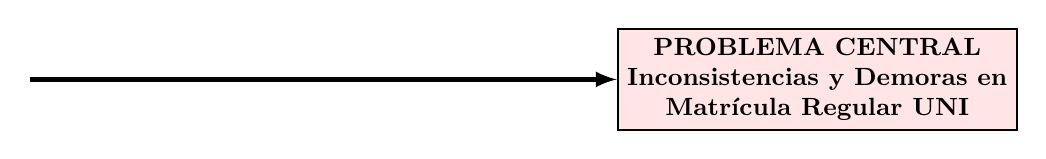
\begin{tikzpicture}[
    >=latex, thick,
    efecto/.style={draw, rectangle, fill=red!10, minimum width=3.8cm, minimum height=1.2cm, align=center, font=\bfseries\small},
    categoria/.style={draw, rectangle, fill=blue!10, rounded corners, text width=3.2cm, align=center, font=\bfseries\small},
    causa/.style={draw=none, inner sep=2pt, font=\scriptsize, align=right, text width=5cm}, 
    punto/.style={circle, fill=black, inner sep=1.5pt}
]

    % EJE CENTRAL Y PROBLEMA CENTRAL
    \node[efecto] (P) at (10,0) {PROBLEMA CENTRAL\\Inconsistencias y Demoras en\\Matrícula Regular UNI};
    \draw[ultra thick, ->] (0,0) -- (P);

    % PUNTOS DE CONEXIÓN EN EL EJE CENTRAL
    \path (0,0) -- (P.west)
        coordinate[pos=0.3] (S1)
        coordinate[pos=0.9] (S2);

    % ESPINAS SUPERIORES
    \espina{SUB1}{S1}{4.6}{Subproceso 1:\\Acreditación y\\Pre-requisitos}{
        \addcausa{0.35}{Falta de integración en tiempo real del control de deudas}
        \addcausa{0.75}{Retraso manual en fichas de reincorporados y convalidados}
    }

    \espina{SUB2}{S2}{4.6}{Subproceso 2:\\Selección y\\Registro de Cursos}{
        \addcausa{0.20}{Saturación y caídas en portal DIRCE por alta concurrencia}
        \addcausa{0.42}{Agotamiento acelerado de vacantes en secciones clave}
        \addcausa{0.64}{Cruces horarios entre asignaturas de ciclos contiguos}
        \addcausa{0.85}{Errores de plan de estudios y prioridad de egresados}
    }

    % ESPINAS INFERIORES
    \espina{SUB3A}{S1}{-4.6}{Subproceso 3.A:\\Verificación de\\Reglas Académicas}{
        \addcausa{0.35}{Detección tardía de Grupo Cero/sanciones por actas pendientes}
        \addcausa{0.75}{Sobrecarga por procesamiento manual de rectificaciones}
    }

    \espina{SUB3B}{S2}{-4.6}{Subproceso 3.B:\\Confirmación y\\Registro Oficial}{
        \addcausa{0.25}{Falta de autonomía de Facultad para cambios en DIRCE}
        \addcausa{0.55}{Desfase entre alumnos asistentes y padrones docentes}
        \addcausa{0.82}{Demoras en el visado de boletas y reporte a SUNEDU}
    }

\end{tikzpicture} 
}
\caption{Diagrama de Ishikawa - Inconsistencias y Demoras en la Matrícula Regular de la UNI.}
\label{fig:ishikawa}
\end{figure}

\subsubsection{Problemática en el Subproceso 1: Acreditación y Pre-requisitos}
El Subproceso 1 busca verificar el pago de autoseguro, la ausencia de deudas y la asignación del turno de matrícula. Identificamos dos fallos principales en la plataforma:
\begin{itemize}
\item \textbf{Falta de integración en el control de deudas:} Aunque el TUPA exige no tener deudas de libros o materiales con la Facultad, la Intranet DIRCE no consulta las bases de datos de biblioteca en tiempo real. Esto permite que alumnos con adeudos se matriculen solo pagando el autoseguro, saltándose la regla de negocio del proceso.
\item \textbf{Rigidez en la actualización de la ficha de matrícula:} Los estudiantes con convalidaciones, exoneraciones o reincorporaciones aprobadas no figuran en la base de datos inicial de la DIRCE. Al depender de un trámite manual para actualizar su estado, el sistema no les libera la ficha a tiempo y pierden su turno de inscripción.
\end{itemize}

\subsubsection{Problemática en el Subproceso 2: Selección y Registro de Cursos}
El Subproceso 2 es la etapa central de la matrícula, donde el estudiante ingresa al portal DIRCE en su turno asignado para armar su horario, elegir secciones y reservar vacantes según el límite de créditos autorizado por su promedio. Sin embargo, este subproceso concentra la mayor densidad de incidencias reportadas durante cada periodo de matrícula. El agotamiento acelerado de vacantes en secciones de alta demanda, la saturación del portal DIRCE por alta concurrencia simultánea, los cruces horarios estructurales entre asignaturas de ciclos contiguos y la omisión de cursos en la interfaz del sistema son problemas recurrentes que afectan a un porcentaje significativo de la comunidad estudiantil. Estas fallas no son solo técnicas, sino que responden a debilidades en la articulación entre la lógica del proceso de negocio y la capacidad del sistema de información que lo soporta, tal como establece la distinción conceptual entre proceso y sistema.

\subsubsection{Problemática en el Subproceso 3.A: Verificación y Control de Reglas Académicas}
El Subproceso 3: Verificación y Control de Reglas Académicas es la etapa posterior inmediata a la generación de la pre-ficha de matrícula y reserva temporal de cupos del Subproceso 2. Consiste en la fiscalización, validación y control riguroso de la selección preliminar de asignaturas efectuada por el estudiante en la plataforma Intranet DIRCE/SIGA-ORCE. Su propósito central es verificar que la carga lectiva solicitada cumpla estrictamente con la normativa universitaria y las directivas internas (límites de créditos por promedio ponderado, prelaciones, cursos de arrastre/repitencia, planes curriculares vigentes y condiciones académicas especiales) antes del asiento transaccional definitivo del sub proceso 3.b.

\subsubsection{Problemática en el Subproceso 3.B: Confirmación y Registro Transaccional Oficial}
La etapa de cierre del proceso presenta deficiencias operativas observables. Durante la primera semana de clases, la Oficina de Estadística de cada Facultad aún está registrando matrículas rezagadas de reincorporados y procesando reducciones, adiciones y cambios de asignaturas aprobados por la Dirección de Escuela (Reglamento de Matrícula, RR. N.° 570-2022, Art. 77°), lo que produce un desfase entre lo que ocurre en las aulas y lo que figura en las nóminas provisionales: estudiantes que asisten a cátedra sin aparecer en los listados de sus docentes. A ello se suman las demoras en el visado del Reporte y de la Boleta de Matrícula por la sobrecarga de trabajo de las Oficinas de Estadística (documento exigido para trámites de becas, seguros y otros), las inconsistencias en la migración de datos hacia SUNEDU que retrasan la validación del padrón nacional y la expedición del carné universitario, y una concentración de operaciones manuales y repetitivas en la etapa de consolidación y cierre. A estas deficiencias se añade la más severa reportada en el proceso 2026-2: la Facultad carece de acceso directo al sistema para realizar modificaciones de matrícula (por ejemplo, ajustes de horarios acordados con alumnos y docentes), de modo que toda corrección depende de trámites ante la Dirección de Registro Central y Estadística (DIRCE), con la pérdida de oportunidad que ello implica.

Esta situación afecta, en primer lugar, a los estudiantes, que inician el ciclo sin documentación oficial oportuna y con riesgo de no figurar en los padrones de sus asignaturas; a los docentes, que reciben listados incompletos o desactualizados para el registro de asistencia y evaluación; al personal administrativo de las Oficinas de Estadística y de la DIRCE, sobrecargado de reprocesos en plazos improrrogables; y a la propia universidad, cuya posición frente a los organismos supervisores depende del cumplimiento de plazos normativos estrictos, como la remisión de reportes a SUNEDU y MINEDU en un máximo de veinte días (Art. 79°) y la disposición del registro y las boletas de matrícula a las Facultades en un plazo no mayor de diez días hábiles tras el cierre (Art. 80°). Por tratarse del eslabón final de la cadena, el subproceso sufre además el efecto acumulado de los subprocesos anteriores: los rezagos de habilitación, convalidación y rectificación que no se resolvieron aguas arriba aterrizan en la semana de verificación y en el cierre, donde se manifiestan como desfase de padrones y reproceso manual. La consecuencia global es la pérdida de oportunidad, confiabilidad y trazabilidad de la información académica precisamente en la ventana más crítica del semestre.